\chapter{Computational Methods}
\label{chap:comp_methods}

In physics, the ultimate goal is to derive a solution from fundamental postulates (first-principles) whose predictions match with empirical observations. However, what it means to `solve' a system, depends on the techniques applied. As an example, shown in Table  \ref{table:types_of_physics_solutions} are some canonical variables sought after in various sub-fields of physics.
\begin{table}[!h]
  \begin{tabular}{l|l|l}             
    Classical Mechanics & $\qp (t)$ & Positions and momenta as functions of time \\
    Quantum  Mechanics  & $\psi$ & Wave-functions \\
    Fluid Dynamics & $\B{v}$ & Velocity fields of the flow\\
    Chaos Theory & $\lambda$, $\text{D}_\alpha$ & Lyapunov exponents, fractal dimension \\
    Statistical Mechanics & $\Z$,  $\Omega$ & Partition functions, density of states
  \end{tabular}
  \caption{}
  \label{table:types_of_physics_solutions}
\end{table}
While the list is necessarily incomplete and inherently subjective, it illustrates how different each solution can be. Each subfield has its own approximations and limits; it is important that the predictions made are understood within the correct scope. Hence we want to be clear what limits we wish to impose in our present discussion. In the context of this thesis, we concentrate mainly on equilibrium distributions from statistical mechanics and dynamics (kinetics) derived from those results.

The foundations of Statistical Mechanics historically come from thermodynamics, the study of temperature and heat. Entire treatises, books and journals are dedicated to the topic, for the reader interested in a historical background see Lewis.\cite{lewis_heat_2007} There are three (+1) laws of thermodynamics, the zeroth law so named for the connection to commutativity axiom.  \newline
\epigraph{
  \begin{itemize}
  \item Zeroth Law : If system $\mathcal{B}$ is in thermal contact and equilibrium with systems $\mathcal{A}$ and $\mathcal{C}$ then $\mathcal{A}$ must be in thermal equilibrium with $\mathcal{C}$. 
  \item First Law : If system $\mathcal{A}$ is isolated, then total energy remains constant. It can however, change forms.
  \item Second Law : In a closed system, the result of any irreversible process must increase entropy, and remain constant for a reversible process; $S \ge 0$
  \item Third Law : The entropy of a system approaches zero as the absolute temperature goes to zero.
  \end{itemize}
}{The Laws of Thermodynamics}

The primary consideration of this thesis is the study of entropy involved in the protein folding process. Underpinning all of the discussions in the subsequent chapters is the idea of a canonical ensemble from statistical mechanics. As such, we feel that its derivation from the Hamiltonian under suitable restrictions, is paramount to the ideal of a complete and self-contained thesis. Much of the material in the Section \ref{sec:stat_mech_intro} is adapted from several of the notable statistical mechanics texts, namely Pathria,\cite{pathria_statistical_1996} Kittel\cite{kittel_thermal_1980} and Dill.\cite{dill_molecular_2002}

\section{Statistical Mechanics}
\label{sec:stat_mech_intro}

Statistical mechanics is a more abstract representation of a system then the physical quantities considered in thermodynamics. Indeed the notion of temperature and states do not have to correspond to directly physically observable quantities (\cf Shannon's information theory\cite{shannon_mathematical_2001}). With the advent of statistical mechanics the three laws of thermodynamics can be formulated from a more fundamental postulate, from which some of the above laws of thermodynamics can be derived. \newline
\epigraph{
  \begin{itemize}
  \item Given an isolated system in equilibrium with a finite number of microstates $\Omega$ of equal energy, the probability of finding the system in any particular microstate is $1/\Omega$.
  \end{itemize}
}{The Fundamental Postulate of Statistical Mechanics}

We begin with the Hamiltonian, arguably the most fundamental quantity in all of physics. 
Let us consider $N$ particles and their instantaneous position $q_i(t)$ and momenta $p_i(t)$ where $i=1 \ldots N d$ and $d$ is the dimension of the system. We refer to these coordinates 
$\qp = (q_1, q_2, \ldots, q_{Nd}, p_1, p_2, \ldots, p_{Nd})$ as a microstate of the system. The Hamiltonian $\HAM \qp$ gives a set of $d$ coupled differential equations that govern the dynamical behavior of the system. We refer to this $d$-dimensional space of coordinates $\qp$ as the phase space of the system. The evolution of the system through phase space is given by the canonical relations
\begin{align}
  \dot q_i &=  \pfrac{\HAM \qp}{p_i}  \\
  \dot p_i &= -\pfrac{\HAM \qp}{q_i} 
\end{align}
It is worth noting at this point that, if the system is known to have a fixed energy
\begin{equation}
  \HAM \qp = E
\end{equation}
then the system will trace out a trajectory in phase space that is restricted to a hypersurface of dimension $d-1$ (if there are no other constants of motion). 
%While it is mathematically valid to consider systems whose Hamiltonian traces out trajectories that fill unbounded regions of phase space, we often restrict ourselves to Hamiltonians that fill only a bounded region of the space. An unbounded system which does not conserve energy, is certainly unphysical in the context of most real systems, biophysics included. 
The phase space splits naturally into two regions, allowed and disallowed, whose particulars depend on the form of the Hamiltonian and the initial conditions. Considering all points in the allowed region, we can form a (possibly time-dependent) density function $\rho(\B{q},\B{p}; t)$ which determines the number of microstates are found in a given volume of phase space
\begin{equation}
  \rho(\B{q},\B{p}; t) \, d \B{q} \, d \B{p}
\end{equation}
%
In the context of this thesis, we will consider only density functions that are stationary
\begin{equation}
  \pfrac{\rho(\B{q},\B{p})}{t} = 0
  \label{eq:stationary_conditions_density_function}
\end{equation}
which correspond to systems in equilibrium. Under the assumptions of equilibrium, powerful results can be derived. Since the phase space does not admit ``sources'' or ``sinks'', \ie  the total number of points must be conserved, the total inflow and outflows must be the same over time. Letting $\omega$ represent an arbitrary volume in phase space and $\B{v}$ be the velocity vector of the points in phase space we get
\begin{equation}
  \pfrac{\rho}{t} + \nabla \cdot \rho \B{v} = 0
\end{equation}
which is simply the continuity equation of the system. This is a conservation of the phase space volume, but the generic form is common throughout physics (for example, a similar expression can be found implicitly in Maxwell's equations (\cf Jackson\cite[page 3]{jackson_classical_1998}) for the continuity of charge and current density). Manipulating them further, one can get Louisville's theorem \cite{liouville_1985}
\begin{equation}
  \frac{d \rho}{d t} = \pfrac{\rho}{t} + [\rho, H]
\end{equation}
where the Poisson bracket $[ \rho, H ]$ is defined as
\begin{equation}
  [ \rho, H ] =
  \sum_{i=1}^{d}
  \pfrac{\rho}{q_i}
  \pfrac{H}{p_i}
  -
  \pfrac{\rho}{p_i}
  \pfrac{H}{q_i}
\end{equation}
According to this theorem, if one could travel along with a group of points, one would find that the local volume of points remains constant. Using the equilibrium condition from Equation \ref{eq:stationary_conditions_density_function} we have the restriction
\begin{equation}
  [ \rho, H ] = 0.
  \label{eq:phase_space_equlibrium_condition}
\end{equation}


\subsubsection{Ensembles}
\label{sec:ensemble}

There is more then one way to satisfy the restriction in Equation 
\ref{eq:phase_space_equlibrium_condition}, the choice of which leads to the various statistical ensembles. It is convenient to define a macrostate which is a collection microstates that share common aggregate values. We let the particle number $N$, volume $V$ and energy $E$ of a system define a macrostate by the tuple $(N,V,E)$, with the number of available microstates in a given macrostate as $\Omega(N,V,E)$. 

Placing two systems $\Omega_1(N_1,V_1,E_1)$ and $\Omega_2(N_2,V_2,E_2)$ with a hard but thermally conductive barrier at thermal equilibrium would settle to a composite state $\Omega_3$. In full generality we can set $E_1=0$ as a reference point and $E_2>0$. Conservation laws tell us that the total volume, particle number and energy are simply $V_3=V_1+V_2$, $N_3 = N_1+N_2$, $E_3 = E_1+E_2$ but the question remains, how much energy is transferred from the second system to the first? The second law of thermodynamics tells us how this is done. The final number of states 
$\Omega_3(N_3,V_3,(E_1, E_3))$ is maximized. The rationale behind such an assumption is generally considered valid as, from a purely probabilistic standpoint, the most likely state must be the most common. In addition, the next most probable state is often orders of magnitude less likely then the first, making this specific choice of $\Omega_3$ to correspond to the state at which the system spends ``most'' of its time in. It is natural then, to identify this state with the equilibrium of the system. We find that the subsystems exchange energy until this point is reached, and hence by the zeroth law of thermodynamics, they must share a common parameter (which we call $\beta$ for now)
\begin{equation}
  \beta \equiv \paren{
    \pfrac{\ln \Omega(N,V,E)}{E}
  }
  _ {N,V,E=E_{\text{eq}}}
  \label{eq:stat_basis_eq1}
\end{equation}
From the thermodynamic relation
\begin{equation}
  \paren{
    \pfrac{S}{E}
  } _ {N,V} = \frac{1}{T}
  \label{eq:stat_basis_eq2}
\end{equation}
and Equation \ref{eq:stat_basis_eq1} we find that
\begin{equation}
  \pfrac{S}{\ln \Omega} = \frac{1}{\beta T} = \text{const.}
\end{equation}
This is identified as the Boltzmann constant, which is related to the gas constant $R$ and Avogadro's number $N_A$
\begin{equation}
  k_B=R/N_A=1.3806503 \cdot 10^{-23} \frac{\text{m}^2 \text{kg}}{ \text{s}^{2} \text{K}}
\end{equation}
This implies the famous relation first discovered by Boltzmann
\begin{equation}
  S = k \ln \Omega
\end{equation}
a relation between the entropy and the number of states of the system. 

We consider first the microcanonical ensemble, where the particle number $N$, volume $V$ and energy $E$ are all fixed quantities,\footnote{One could also consider the case when the energy lies within a fixed \textit{range} instead $E_0 -\Delta \le E \le E_0 +\Delta$, but the same difficulties will still arise in this formulation.} of all the ensembles considered this is the most restrictive. In the microcanonical ensemble all states in phase space are equally likely, such that Equation \ref{eq:phase_space_equlibrium_condition} is satisfied by
\begin{equation}
  \rho \qp = \text{const.}
\end{equation}
This postulate is commonly referred to as ``equal \textit{a priori} probabilities''. The equilibrium condition can be satisfied in a more general way, such that the dependence of $\rho$ depends only explicitly on the Hamiltonian. The more general restriction for a stationary ensemble provides a class of density functions. We will see that the class where $\rho \qp \propto \exp ( c H \qp )$  is of particular importance.

The microcanonical ensemble becomes unsatisfactory when considered from a realistic experimental standpoint. For one, it would be hard to keep a real experiment at constant energy. In addition there are few realistic systems in which one can measure the energy \textit{directly}. A more common scenario is to imagine our system of interest to be kept at constant temperature by coupling it with a large reservoir. Let the large reservoir be system $A$, and the smaller system of interest be system $B$ with macrostate parameters $(E_A, T)$ and $(E_B, T)$ respectively. The energy of the smaller system would be in flux over time and could range from zero to the composite energy of the system $E_{AB} = E_A + E_B = \text{const}$. However, since the reservoir system contains many more states then the smaller one, and that probability of each microstate at a fixed energy is equal, the probability of any given energy value of the smaller system must be proportional to
\begin{equation}
  P(E_B) \propto \Omega(E_A) \equiv \Omega(E_{AB} - E_B)
\end{equation}
We can carry out a Taylor series expansion of the above around the value of $E_A = E_{AB}$ \ie $E_B=0$. For reason of convergence we do so around the logarithm instead, giving
\begin{equation}
  \ln \Omega (E_A) = \ln \Omega(E_{AB}) + 
  \paren{
    \pfrac{\ln \Omega}{E'}
  }
  _ {E' = E_{AB}}
  (E_A - E_{AB}) 
  + \ldots
\end{equation}
At equilibrium and from Equation \ref{eq:stat_basis_eq1} we get the fundamental relation for the canonical ensemble
\begin{equation}
  P(E_B) \propto \exp (-\beta E_B)
  \label{eq:cannonical_prob_unnormal}
\end{equation}

To normalize Equation \ref{eq:cannonical_prob_unnormal} we simply divide by all possible energy levels. This `sum over all states function', plays particular importance in studies carried out in this thesis as it essentially (along with the density of states) provides all the thermodynamic information of the system. In language of equilibrium thermodynamics, it is known as the partition function $\Z$ (German: \textit{Zustandssumme}). The partition function then, is the sum of all the events that could occur weighted with their probability over the canonical ensemble. If, as in many physical cases, the energy levels of the system are degenerate, the sum is modified by this multiplicative factor as well. If we let $g(E_i)$ be the degeneracy of energy level $E_i$ one has
\begin{equation}
  \Z = \sum_{E_i} g(E_i) \exp(-\beta E_i)
\end{equation}
%
From this we state the general thermodynamic relations from the canonical ensemble (see \citealt[page 53]{pathria_statistical_1996}). With $P$, $U$, $S$, $T$, $A=U-TS$ as the probability, internal energy, entropy, temperature and Gibbs free energy respectively we have
\begin{align}
  P(E_i) &= g(E_i) \exp( - \beta E_i ) / \Z \\
  U &= \sum_{E_j} E_j g(E_i) \exp( - \beta E_j ) / \Z \\
  A &= -k T \ln \Z \\
  S &= -k \sum_{E_j} P(E_j) \ln P(E_j)
\end{align}
The last relation is the most interesting. The implication is that, if we had complete knowledge of the energy level degeneracies $g(E)$, all thermodynamic variables could be computed. The function $g(E)$, up to a normalization constant is known as the density of states. We shall see in Section \ref{sec:wang_landau} that specialized numerical algorithms have been devised that determine this function to high accuracy.

There are physically relevant limits at which the system reduces to particularly simple forms. At high enough temperatures we find that the steady-state distribution is simply the sum over the degeneracy term, $g(E)$
\begin{equation}
  \lim_{T\rightarrow \infty} \Z = \sum_{E_i} g(E_i) 
\end{equation}
and at low temperatures the system is dominated by the ground state
\begin{equation}
  \lim_{T\rightarrow 0} \Z = g(E_1)  \exp(-\beta E_1)
\end{equation}.

For completeness, we mention a third ensemble, the grand canonical ensemble. In this ensemble, both the energy and the particle numbers are allowed to be exchanged from the reservoir to the smaller system. In this case both the temperature $T$ and the chemical potential $\mu$ are fixed giving the equilibrium distribution distribution relation as
\begin{equation}
  P(E_B, N_B) \propto \exp ( -\alpha N_B - \beta E_B)
\end{equation}
where
\begin{equation}
  \alpha = - \frac{\mu}{kT}
\end{equation}
The fugacity of the system is $z = \exp(-\alpha)$. While not explicitly used in this thesis, many of the models presented have obvious extensions to allow a variable particle (or in our case protein) count. A sampling method to determine the density of states would have to count system conformations $g(E_i, N_j)$ but the extension is natural.

\subsubsection{Example three-level system}

To demonstrate the concepts, we will use a sample system with the energy levels shown in Figure \ref{fig:sample_energy_level}. In this system there are three discrete energy levels ($E_1=-4$, $E_2=-2$, $E_3=0$) with a state degeneracy of $g(E_1) = 1$, $g(E_2) = 2$, $g(E_3)=5$.
%
\begin{figure}
  \TIKZenergylevel
  \caption{Sample three-level system with degeneracy levels shown.}
  \label{fig:sample_energy_level}
\end{figure}
%
The partition function is
\begin{equation}
  \Z = e^{4\beta} + 2 e^{2\beta} + 5 
\end{equation}
%
Giving the probability of each state
\begin{align}
  P(E_1) &= \frac{e^{4\beta}}{\Z}  \\
  P(E_2) &= \frac{2 e^{2\beta}}{\Z}  \nonumber \\
  P(E_3) &= \frac{5  e^{0 \cdot \beta} }{\Z} = \frac{5}{\Z} \nonumber
\end{align}

A plot of the probabilities and the corresponding specific heat in units of $1/\beta=kT$ are shown in Figure \ref{fig:sample_energy_prob}. The peak in the specific heat is a nice example of the so-called Schottky anomaly,\cite{schottky_zur_1922} as normally the specific heat is monotonically increasing with temperature. In this case however, the peak corresponds to a loose `melting' of the system, when the system undergoes a transition from a full occupancy of the ground-state to the general disordered state found at high temperatures. In this case, since the number of energy levels are very small, the effect is small and correspondingly the peak is quite broad. We will see more physically relevant examples with sharper peaks in the later chapters when we consider larger systems.
%
\begin{figure}
  \subfloat[$P(E)$]{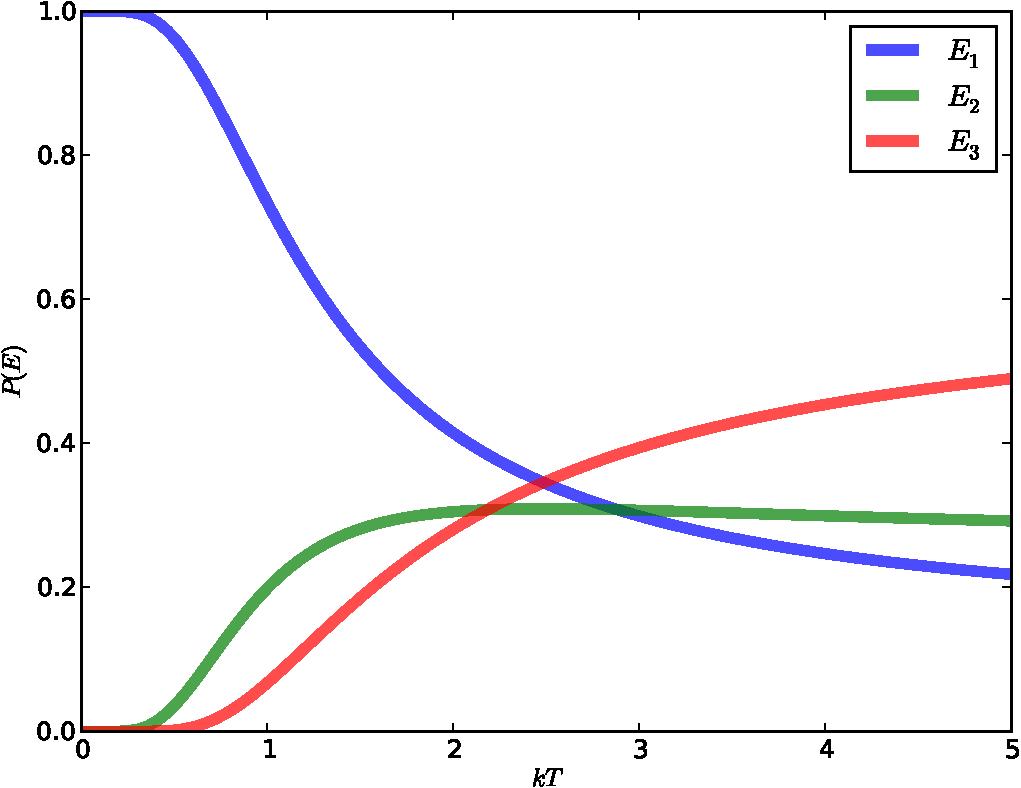
\includegraphics[width=.45\textwidth]{pictures/three_level_system/three_level_E-crop.pdf}}
  \subfloat[$C_V$]{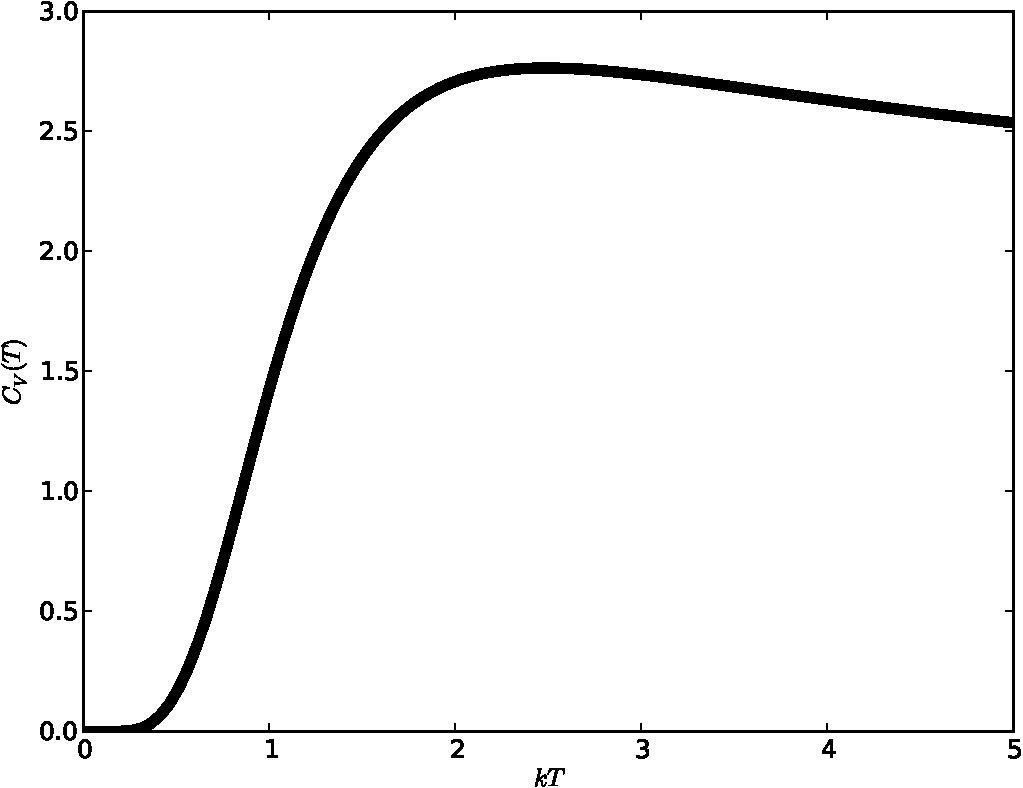
\includegraphics[width=.45\textwidth]{pictures/three_level_system/three_level_CV-crop.pdf}}
  \caption{Probabilities for each state of the sample three-level system (see Figure \ref{fig:sample_energy_level}) and the specific heat as a function of $1/\beta=kT$. }
  \label{fig:sample_energy_prob}
\end{figure}

%-------------------------------------------------------------------------------------

\section{Monte Carlo Methods}
\label{sec:monte_carlo}

In statistical mechanics we are not integrating a set of differential equations (as one would in the Classical or Quantum), but determining the distribution that satisfies the steady-state properties of a given Hamiltonian at a specific temperature. If the system is small and enumerable, such as the one we encountered in Section \ref{sec:ensemble}, we can evaluate the exact form of $\Z$. If the system displays self-similarity such as the Ising/Potts models 1D, 2D or over Cayley trees sometimes an analytical solution can be found.\cite{wu_potts_1982} In general however, the size state-space is too large and complex (and in the continuous case, too rough to discretize at a reasonable level) to completely solve for the states of the system. In general, one must use sampling methods to solve for the distribution. The etymology of the phrase `Monte Carlo' connects the random sampling of a physical system with the games of chance (whose profits also rely on random distributions) in the celebrated city of the same name in Monaco. 

\subsection{Metropolis-Hastings}
\label{sec:metroplis_hastings}

While many different adaptations of a Monte Carlo exist, the method most often used in physics simulations is the Metropolis-Hastings.\cite{metropolis_equation_1953} The Metropolis-Hastings algorithm is essentially a Markov transition matrix (a concept fully explained in Section \ref{sec:markov_matrix}). For each pair of valid conformations $(\xi_A, \xi_B)$ of the system (which need not be finite), there exists a corresponding matrix element that represents the transition probability. Not every state has to be connected to every other state, the only requirement is that connections between the conformations are ergodic, in that eventually every state will be reached from every other state. There exists a function called the move set which relates, from a given state, the accessible states to it.

The full Metropolis Hastings algorithm is a more general method of sampling then will be presented here, which will be confined to the simulation of physically relevant numerical experiments. From the canonical ensemble, the probability of observing a single conformation is $P(\xi_A) = \exp(-\beta E_A) / \mathcal{Z}$. When considering the ratio of two states, the partition function cancels leaving
\begin{equation}
  P(\xi_A \rightarrow \xi_B) = \frac{ \exp(-\beta E_A) } { \exp(-\beta E_B) } = \exp(-\beta \Delta E)
  \label{eq:metroplis_hastings_formula}
\end{equation}
with $\Delta E = E_A - E_B$. Hence, by using a move set function and starting from an initial conformation $\xi_0$ one proceeds to sample the state space by accepting or rejecting new conformations based on the probability in Equation \ref{eq:metroplis_hastings_formula}. 

This method, and others like it, generate a canonical distribution at a fixed temperature. The primary disadvantage is the lack of data over a significant range of temperatures, making multiple simulations necessary for the calculation of thermodynamic quantities. At low temperatures the algorithm can get stuck in local minima, severely impacting convergence rates. Various methods have been proposed to counteract this shortcoming, simulated annealing\cite{kirkpatrick_optimization_1983} being the most popular. In addition, near phase transitions the system can exhibit a critical slowing down, making the convergence extremely slow.\cite{yahata_critical_1969} 

\subsection{The Wang-Landau Density of States Method}
\label{sec:wang_landau}

Wang-Landau (WL) sampling\cite{wang_determining_2001} is a generic algorithm to calculate the relative density of states (DOS) for a given system. The algorithm starts off with the initial \textit{a priori} \textit{ansatz} that all conformational states are equally likely $\Omega(\xi)=1$, where $\xi$ is a conformation of the system.  Traditionally the calculation of the density of states was computed as a function of the energy of the system. Like others, we extend the use the Wang-Landau method to determine the the density of states for a set of conformations of the system rather than the energy explicitly.\cite{patel_effect_2008, wust_versatile_2009} This allows the system to be sampled for all values of the free variables simultaneously as the conformations can be turned into energies later.

In the WL method, the density of states is iteratively refined, crudely at first to ensure a large sampling, and then with greater precision as $\Omega$ converges. Similar to a typical Monte-Carlo simulation the algorithm has an acceptance rate. However, unlike traditional Metropolis-Hastings simulations, the process can not be modeled as a Markov chain since the transition matrix itself is iteratively refined. The WL acceptance rate is
\begin{equation}
  P(\xi_A \rightarrow \xi_B) = \min 
  \paren{ 
    1, \frac{\Omega(\xi_A)}{\Omega(\xi_B)} \frac{n_{B \rightarrow A}/n_B}{n_{A \rightarrow B}/n_A} 
  }
\end{equation}
Where $n_A$ is the number of outgoing moves from states $A$ and $n_{A \rightarrow B}$ is the number of moves from $A$ to $B$ (similarly defined for $n_B$ and $n_{B \rightarrow A}$). If the moves are reversible then $\frac{n_{B \rightarrow A}}{n_{A \rightarrow B}}=1$. These factors are necessary for detailed balance if the move set chosen has a variable number of moves from each state. Once any particular state had been selected the density of states is modified by $\Omega(\xi) \rightarrow f\Omega(\xi)$ where $f$ is a constant that is slowly reduced to unity during the simulation. 

It is important to note that the process is iterative, which has its advantages and disadvantages. Since the process uses the previous value of the density of states to determine the next refinement, excellent speedups can be obtained if one has any prior information about the distribution of the conformational degeneracies of the system. This may come from a previous simulation or general knowledge (for example, the 2D Ising model is roughly quadratic in log space). However, unlike the traditional Metropolis-Hastings models, the iterative refinement of the density states makes the process unable to be mapped to a Markov chain. This severely limits the analytic treatment that can be applied when discussing the convergence rates and saturation of errors. Several adaptions have been proposed to improve the algorithm. One can minimize the saturation of errors using an N-fold way process\cite{belardinelli_wang-landau_2007} with a steadily decreasing constant. One can also modify the move set in an optimal way to improve convergence.\cite{wu_overcoming_2005}

If the state space is not discrete, additional considerations have to be made. For the algorithm to generate a histogram, the continuous state space has to be discretized. Without prior knowledge of the system this can be difficult. If the level spacing is to small then the algorithm may fail to converge in a reasonable amount of time. If the level spacing is too large it may obscure the results, especially where the derivative of the density of states is large. To partially mediate the problem, we provide an approximation to the specific heat (a typically sought after parameter) in Appendix \ref{chap:macrostate_approx}.

%----------------------------------------------------------------------------------------

\section{Networks and Graphs}
\label{sec:graph_introduction}

This section introduces the idea of a graph. A graph $G$ is a collection of vertices $\{v_1, v_2, v_3, ...\} \in \mathcal{V}$ and edges $\{e_1, e_2, e_3, ...\} \in \mathcal{E}$. An edge is defined by the two vertices connecting to it, $e_i = (v_a, v_b)$. If the graph is directed then the ordering matters, \ie  the edge $(n_a, n_b)$ points only from $n_a$ to $n_b$. If the graph is undirected then the an edge is considered to point both ways. The edge set $\mathcal{E}$ for a graph contains only unique entries, as opposed to multi-graphs where this restriction is relaxed. Edges can carry a weight which we associate with each edge $\{e_1 : w_1, ..., e_i : w_2\}$. A vertex can also have a weight, and is associated the same way, $\{v_1 : n_1, ..., v_i : n_2\}$. If a graph has an edge connection to itself $e_i = (n_j, n_j)$ this edge is called a loop. Undirected, loop-free graphs are called simple graphs.

A useful device for keeping track of graphs is the adjacency matrix. In this matrix, the non-zero entries are those where an edge connects vertices $v_i$ to $v_j$
\begin{displaymath}
  \B{A}_{ij} = \piecewisebrace{
    \begin{array}{l r l}
      1 & : & e_k = (v_i, v_j) \in \mathcal{E}\\
      0 & : & \text{otherwise}
    \end{array}
  }
\end{displaymath} 
%
As an example, see Figure \ref{fig:example_graph_5node}, for a simple graph whose adjacency matrix is
\begin{equation}
  \B{A} = 
  \begin{bmatrix} 
    0 & 0 & 1 & 0 & 0 \\
    0 & 0 & 1 & 0 & 0 \\
    1 & 1 & 0 & 1 & 1 \\
    0 & 0 & 1 & 0 & 1 \\
    0 & 0 & 1 & 1 & 0 \\
  \end{bmatrix}
  \label{eq:example_graph_5node}
\end{equation}
\begin{figure}[ht]
  \begin{center}
    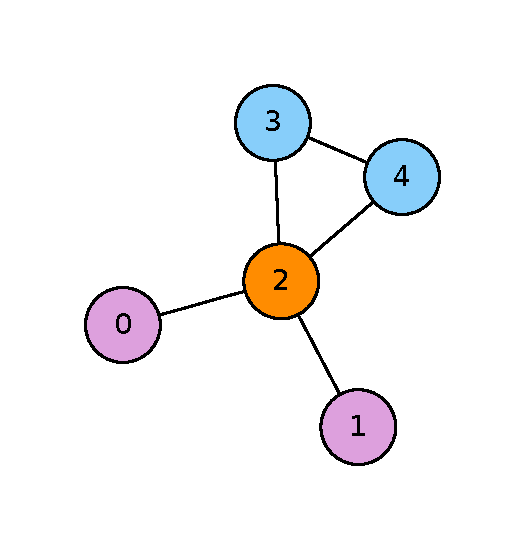
\includegraphics[width=\figurewidthTRIPLE]{pictures/graph_examples/example_simple_graph.pdf}
  \end{center}
  \caption{ 
    Pictorial representation of the graph given by the adjacency matrix, Equation \ref{eq:example_graph_5node}. The vertices are colored according to the walking polynomial defined in Equation \ref{eq:walking_polynomial}. }
  \label{fig:example_graph_5node}
\end{figure}
%
The adjacency representation is computationally useful, with it various graph properties can be calculated with ease. For example, one can show that $(\B{A}^2)_{ij}$ is the number of paths from $v_i$ to $v_j$ in exactly two steps. This holds in general, $(\B{A}^n)_{ij}$ is the number of paths from $v_i$ to $v_j$ in exactly $n$ steps. This connection between repeated iterations of multiplication makes simple graphs a natural study in the context of Markov matrices. 

\subsection{Graph Operations}
We will find it useful to perform two specific operations on the structure of the graph itself. The first, \emph{edge removal}, is simple. We define the operation $G_{-e_{ij}}$ to be the graph constructed from the edge set of $G$ with the edge $(v_i, v_j)$ removed. It is worthwhile to note that edge removal may split the graph into two disconnected subgraphs. If this happens we denote the subgraphs $G_1$ and $G_2$ as $G_{-e_{ij}} = G_1 \sqcup G_2$. The second operation, \emph{edge contraction}, is denoted by $G_{/ e_{ij}}$. In edge contraction vertices $v_i, v_j$ are merged into a new vertex $v_k$. All vertices that previously joined to $v_i$ or $v_j$ are now joined to the new vertex $v_k$. This operation can turn a simple graph into a non-simple one due to the presence of multiple edges. If this is the case, then the graph lacks a nice representation of an adjacency matrix (but it still can be referred to through its edge set $\mathcal{E}$). Representations of the two operations are shown in Figure \ref{fig:example_graph_5node_operations}.
\begin{figure}[ht]
  \begin{center}
    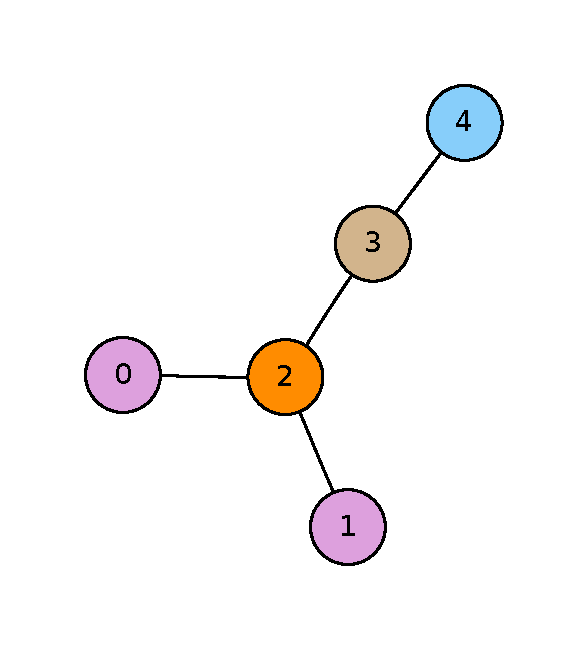
\includegraphics[width=\figurewidthTRIPLE]{pictures/graph_examples/example_simple_graph2.pdf}
    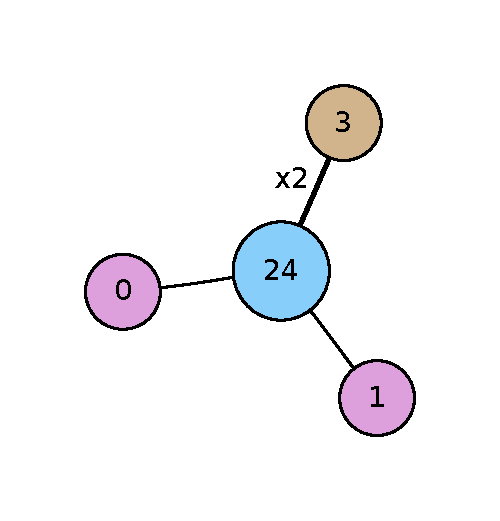
\includegraphics[width=\figurewidthTRIPLE]{pictures/graph_examples/example_simple_graph3.pdf}
  \end{center}
  \caption{Examples of edge removal (left) and edge contraction (right) of the edge $(v_2, v_4)$ on the graph shown in Figure \ref{fig:example_graph_5node}. Each operation removes exactly one edge. In this case edge contraction has made the graph non-simple due to the presence of a multi-edge (indicated by the x2.}
  \label{fig:example_graph_5node_operations}
\end{figure}

\subsection{Graph Isomorphism}
The ability to quickly determine if two graphs are isomorphic has attracted the attention of physicists, chemists, computer scientists and mathematicians for years. It is a long-standing open problem in both pure mathematics and its application. Graph structures are a common theme throughout this thesis, making the study of graph isomorphism relevant to many of the computations. For an approximate answer the problem is considered solved for most cases with the software \textit{nauty}.\cite{mckay_nauty} On a purely theoretical level, the exact solution is unique in terms of computational complexity. It is proposed that the problem is outside of the $\cal{P}$ vs $\cal{NP}$ class.\cite{schoning_graph_1988} Despite the growing number of invariants proposed, the graph isomorphism problem remains unsolved. Its ability to occupy the scientific world has been enough to label it as a plague on the community.\cite{read_graph_1977}

Nevertheless, we propose another invariant, the walking polynomials,  and do so with three goals in mind. The first is to expand upon the arsenal graph theorists have to determine basic properties of a particular graph. The second is the identification that the walking polynomials lend themselves naturally to a coloring scheme that allows the viewer to quickly identify the symmetries of the graph. Finally it is conjectured that the walking polynomials serve as a polynomial-time test to determine if two graphs are isomorphic.

The motivation for the algorithm comes naturally from the study of diffusive processes. The finite limit of a diffusive process is a collection of random walks along a graph. We can count (and solve) for a closed form expression for the number of closed loops along a graph starting at any particular vertex. A generating function can be constructed, one that encodes the path length of \textit{all} walks. It is with these generating functions we construct the invariant known as the walking polynomial.

\subsubsection{Walking Polynomials}
Given a graph with its associated adjacency matrix ${\bf A}$ define 
${\bf S} = ({\bf I} - {\bf A}z)$ and the walking polynomial matrix
\begin{equation}
  {\bf W}(z) = {\bf S}^{-1} = ({\bf I} - {\bf A}z)^{-1}
\end{equation}
%
Which can be computed without taking the inverse via Cramer's rule
\begin{equation}
  {\bf W}_{ij} = \frac{\text{minor}_{ij} {\bf S}} { \text{det} ({\bf S})}
  \label{eq:walking_polynomial}
\end{equation}
The set of diagonal elements $\{ {\bf W}_{11}, {\bf W}_{22}, \ldots, {\bf W}_{nn} \}$ represent the generating functions\footnote{
  It is often the generating functions themselves one is interested in, not any particular term. However, one can extract the $n$\textsuperscript{th} term from the infinite series by differentiating $n$ times to the desired term and setting all higher powers to zero.
  \begin{equation}
    f_{ij}[n](z) =
    \frac{1}{n!}
    \brackets{
      \pfrac{^ n }{ z^n } f_{ij}(z) 
    }
    _{z=0}
    =
    \frac{1}{n!} 
    \brackets{ 
      \pfrac{ ^n }{z^n} \frac{ p_{ij}(z) } { q(z) }
    }
    _{z=0}
  \end{equation}
  %
  If the generating function is a rational function and a closed form is sought, one can perform a partial fraction decomposition. Usually, known relations can reduce the solution to a closed form from this point. In addition, this exposes the poles for asymptotic analysis.
}
for the number of return paths to that vertex. Let an ordered set of these diagonal elements be called $\mathcal{W}$. The choice of ordering is irrelevant, only that it unambiguously sorts rational polynomials. We refer to $\mathcal{W}$ as the walking polynomial for short. We claim that $\mathcal{W}$ is a polynomial time computable invariant.

Take two graphs $G$, $G'$ with adjacency matrices ${\bf A}$, ${\bf A'}$, the matrices ${\bf S}={\bf I}-{\bf A}z$, ${\bf S}'={\bf I}-{\bf A'}z$ and their walking polynomial invariants $\mathcal{W}$, $\mathcal{W'}$. We say that two walking polynomials are equivalent $\mathcal{W} \sim \mathcal{W'}$ if and only if for every $w_i \in \mathcal{W}, v_i \in \mathcal{W}$ we have $w_i = v_i$. By definition, graphs $G$ and $G'$ are isomorphic if and only if there exists a permutation matrix ${\bf P}$ such that
\begin{equation}
  {\bf P A P} ^{-1} = \bf A'
\end{equation}
%
\B{Proof:} \begin{proof}[If $G$ and $G'$ are isomorphic then $\mathcal{W} \sim \mathcal{W'}$] Since $G$ and $G'$ are isomorphic let $\B{P}$ be the permutation matrix ${\bf P A P} ^{-1} = \bf A'$ and $\sigma({\bf P}) \in \{-1, 1\}$ be the the parity of the permutation. The denominator of each of the terms in $\mathcal{W}, \mathcal{W'}$ are related by
  \begin{equation}
    \det({\bf S}) = ({\bf P}) \det({\bf S'})
  \end{equation}
  %
  Given that the permutation matrix maps the numbers $(1, 2, \ldots, N) \rightarrow (k_1, k_2, \ldots, k_N)$ we have
  \begin{equation}
    \text{minor}_{i, i} ({\bf S}) = \sigma({\bf P}) \text{minor}_{k_i, k_i}( {\bf S'} )
  \end{equation}
  %
  Thus for each element $w \in \mathcal{W}$ there must be an element $w' \in \mathcal{W'}$ such that $w = w'$ and hence $\mathcal{W}$ is a graph invariant.
\end{proof}

%----------------------------------------------------------------------------------------


\section{Markov Matrix}
\label{sec:markov_matrix}

A Markov matrix $\B{M}$ is a matrix where each element $\B{M}_{ij}$ describes the probability of a transition from $i \rightarrow j$ in a single time step. As such each row represents a probability distribution
\begin{align}
  \sum_j \B{M}_{ij} & = 1 \\
  0 \leq \B{M}_{ij} & \leq 1
\end{align}

We say that a matrix is positive if all matrix elements are strictly greater then zero $(\forall i,j \hspace{1em} \mathbf{A}_{ij} > 0)$. A matrix is called primitive if there is a $k > 0$ such that $\mathbf{A}^k$ is a positive matrix. Physically, this implies that the matrix becomes well-mixed, and as we will see shortly, allows for the definition of a unique steady-state. If we view the Markov matrix as a graph whose edges are are weighted according to the matrix entries, we see that a disconnected graph implies a non-positive matrix. This typically, is not a problem as the matrix can be broken into separate subgraphs whose solutions are independent. There are however, insidious pathological matrices such as
\begin{equation}
  \B{P} = 
  \begin{bmatrix} 
    0 & 1 \\
    1 & 0 \\
  \end{bmatrix}
  \label{eq:example_non_positive_matrix}
\end{equation}
Here we see that $\B{P}^k=\B{P}$ for all odd $k$, implying that an initial condition in either state will elastically jump and never mix. Connected matrices such as $\B{P}$ are rare in practice however, since a tiny random perturbation to each of the matrix elements $\B{P}_{ij} \rightarrow \B{P}_{ij} + \epsilon_{ij}$ (that preserves the row sums value of unity and keeps all elements non-negative) will force the matrix to become primitive. 

Powers of the matrix describe longer jumps, \ie $(\B{M}^5)_{ij}$ describes the probability of ending up at state $j$ starting at state $i$ after five time steps. The process can be continued indefinitely, but for any primitive matrix, all initial conditions will converge to the same steady state vector. The largest eigenvalue of a primitive Markov matrix is unique and equal to unity, a consequence of the Perron-Frobenius theorem.\cite{perron_zur_1907} Due to the restriction on the row sums, all other eigenvalues are real. The associated eigenvector is then the unique steady-state vector. Intuitively, with only knowledge of the spectra of the eigenvalues, one can deduce this must be so. A large matrix power can be Schur decomposed into a matrix of eigenvectors $\B{V}$ and a diagonal matrix $\B{\Lambda}$ of the eigenvalues by $\B{M}^k = \B{V} \B{\Lambda}^k \B{V}^{-1}$. Since, for diagonal matrices we have $(\B{\Lambda}^k) _ {ij} = (\B{\Lambda}_ {ij})^k$ the appearance of a unique steady-state vector is consequence of the fact that the smaller eigenmodes will decay with time, leaving only the dominant eigenmode.

If the underlying graph of the matrix is disconnected, there will be a multiplicity $k$ in this unit eigenvalue, where $k$ is the number of disconnected pieces in the graph. Since the graph can be permuted into block diagonal form (with $k$ blocks), the degeneracy in the unit eigenvalue corresponds to the unique solution of each separate subgraph.

As an example, let's put weights on our graph (Figure \ref{fig:example_graph_5node}) from the previous section. We will use this matrix as an example to explain the concepts discussed below. To make matters simple, let's assume the probability of leaving (or staying) at any particular vertex is equiproportional, giving us the Markov matrix
\begin{equation}
  \B{M} = 
  \begin{bmatrix} 
    1/2 & 0 & 1/2 & 0 & 0 \\
    0 & 1/2 & 1/2 & 0 & 0 \\
    1/5 & 1/5 & 1/5 & 1/5 & 1/5 \\
    0 & 0 & 1/3 & 1/3 & 1/3 \\
    0 & 0 & 1/3 & 1/3 & 1/3 \\
  \end{bmatrix}
  \label{eq:example_markov_5node}
\end{equation}

As stated, all possible states of the system can be expressed by powers of this matrix. It is useful however to specify a specific state of the system, given as a distribution of over the vertices. For example, consider the initial condition such that all states are localized on vertex $v_1$ (given by the second row of the matrix). We would represent this condition by the vector
\begin{equation}
  \B{v}_0 = [0,1,0,0,0]^T
\end{equation}
One iteration of the Markov matrix with this initial condition would give
\begin{equation}
  \B{M} \B{v}_0 = \B{v}_1 = [0,1/2,1/2,0,0]^T
\end{equation}
And subsequent iterations of the matrix give
\begin{align}
  \B{M}^2 \B{v}_0    &= \B{v}_2  = [1/10,7/20,7/20,1/10,1/10]^T \\
  \B{M}^3 \B{v}_0    &= \B{v}_3  = [3/25,49/200,217/600,41/300,41/300]^T \\
  \B{M}^{50} \B{v}_0 &= \B{v}_5 \approx [.133, .133, .333, .200, .200]
\end{align}
There are a couple of things of interest going on here. The third power of the matrix has strictly positive entries, implying that the matrix is primitive and has a unique steady state distribution. The Schur decomposition is
\begin{align}
  \B{M}           &= \B{V} \B{\Gamma} \B{V}^{-1} \\
  \B{\Gamma}_{ii} &= \{ 1, 0.592, 1/2, 0, -0.225 \}
\end{align}
This appearance of an eigenvalue of unity is not surprising since we know that matrix is primitive. The magnitudes of the other entries set the time-scales for the decay of the other eigenmodes. Even in such a simple system the convergence to steady-state is not monotonic. As we've seen, all modes with $\lambda_i < 1$ are transient and do not effect the steady state distribution. However, the modes close to $1$ may persist for long times (relative to a characteristic time). The state vector $\B{\pi}$, where the net flow away and to each vertex is zero can be stated as the vector satisfying the condition such that
\begin{equation}
  \B{\pi} \B{M} = \B{\pi}
\end{equation} 
\ie the left-eigenvector associated with the unit eigenvalue.

%--------------------------------------------------------------------------------------


\section{Master Equation (ME)}
\label{sec:master_equations}

The master equation is a set of first-order differential equations that describe the time-evolution of a discrete system. It was first introduced by Wolfgang Pauli\cite{pauli_1928_probleme} and later used by Glauber to study the kinetics of the Ising model.\cite{glauber_time-dependent_1963} The master equation relates the change in the probabilities of the occupation of the states $\Xi = \{\xi_1, \xi_2,\ldots, \xi_k \}$ through a vector $\B{p}(t) = [ p_1(t; \xi_1), p_2(t; \xi_2), \ldots] $. From the ME, one can derive many relations used in stochastic dynamics such as the Fokker-Planck equation and Langevin equations. Let the conditional probability of changing from states $\xi_i \rightarrow \xi_j$ be $w_{ij}$. The master equation is
\begin{equation}
  \frac{d}{dt} \B{p}(t) = \sum_{j \neq i} 
  \paren{ w_{ij} \B{p}_j - w_{ji} \B{p}_i }
\end{equation}

The rate of change of the probabilities depends only on the current state of the system, \ie the master equation describes a memory-less or Markovian process. Total probability is conserved
\begin{equation}
  \frac{d}{dt}  \sum_{p_i(t) \in \B{p}(t)} p_i(t) = 0
\end{equation}
%
The master equation can be cast into matrix form
%
\begin{equation}
  \frac{d}{dt} \B{P}(t) = - \B{W} \B{P}(t)
\end{equation}
%
where $\B{W}$ is the stochastic matrix
%
\begin{equation}
  \B{W}_{ij} \equiv
  \piecewisebrace{
    \begin{array}{lr}
      w_{ij}                  & : i \neq j\\
      -\sum_{k \neq j} w_{kj} & : i = j
    \end{array}
  }
\end{equation}
%
By definition the columns sums of $\sum_{i} \B{W}_{ij} = 0$ for all $j$, which is simply a restatement of the conservation of probability. Since the equations are only coupled first-order differentials, their solution is simply
\begin{align}
  \B{P} &= e^{\lambda t} \B{v}  \\
  \B{W} \B{v} &= \lambda \B{v}
\end{align}
%
In general, $\B{W}$ is not symmetric and therefore may have complex eigenvalues. However, any matrix with only real elements is guaranteed to satisfy
\begin{equation}
  \B{W} \B{v} = \lambda \B{v} \rightarrow \B{W} \B{v}^* = \lambda^* \B{v}^*
\end{equation}
Since the elements of $\B{W}$ are always real, the eigenvalues and their associated eigenvectors may be real, or complex conjugate pairs.

For an ergodic system with rate matrix $\B{W}$, the Perron-Frobenius theorem tells us that there is a unique eigenvalue $\lambda_1=0$ and all of the other eigenvalues must have a strictly negative real part. Furthermore the associated eigenvector $\B{v}_1$ must have only non-negative components. This eigenvector has a connection to the steady state probability and ensures that the probabilities are non-negative. All initial conditions of an ergodic system (excluding pathological cases) will approach a steady state vector $\B{\pi}$. A stronger condition is that of detailed balance which holds, if for each pair $i,j$
\begin{equation}
  \B{W}_{ij} \B{\pi} _{j} = \B{W}_{jk} \B{\pi} _{k}
\end{equation}
%
implying that around any closed cycle of states there is no net flow of probability. The master equation has a formal solution
\begin{equation}
  p_i(t) = \sum_{j} \sum_{k} \B{V}_{ik} \exp { \paren{\lambda_k t} } \B{V}^{-1}_{kj} p_j(0)
\end{equation}
%
For a stationary process, \ie a Markovian one, the transition probability depends only on the time interval between two events. Therefore we can write the solution as
\begin{align}
  p_i(t)
  &= [\B{V} \exp { \paren{ {\Gamma t} } } \B{V}^{-1}] p(0) 
  \\ 
  &= \B{M}(t) p(0)
\end{align}
%
Where $\B{M}(t)$ is the matrix exponential of the rate transition matrix. The exponential of a matrix always exists and can be found with a Taylor expansion.
%
\begin{equation}
e ^ {\B{A}} = \B{I} + \B{A} + \frac{1}{2!}\B{A}^2 + \frac{1}{3!}\B{A}^3 + \dots = \sum_{k=0}^{\infty}\frac{1}{k!}\B{A}^k
\end{equation}
If the matrix is diagonalizable it can be found by
\begin{equation}
e^{\B{A}} = \B{V} e^{\B{\Gamma}} \B{V}^{-1}
\end{equation}
Which is trivial since the exponential of a diagonal matrix is
\begin{equation}
\paren{ e^{\B{\Gamma}} } _{ij} = e^{\B{\Gamma}_{ij}} \delta_{ij}
\end{equation}
%
This gives the important relation between a Markov matrix and a rate matrix acting as its generator
\begin{equation}
  \B{M} = \exp(t \B{W}) .
\end{equation}

%---------------------------------------------------------------------------------------
